\documentclass[12pt]{article}
\usepackage[T5]{fontenc}
\usepackage[utf8]{inputenc}
\usepackage{graphicx}
\usepackage{booktabs}
\usepackage{hyperref}
\usepackage[a4paper]{geometry}
\usepackage{fullpage}


\title{Báo cáo Nhập môn Công nghệ phần mềm}
\date{20-12-2014}
\author{
	Nguyễn Việt Hùng - 12520160
	Đỗ Trung Hiếu - 12520135
	Vũ Thành Nhân - 12520302
}

\begin{document}
	\tableofcontents
	\newpage
	%\maketitle
	
	\section{Lời nói đầu}
	Đồ án môn học Nhập môn Công nghệ Phần mềm là phân tích và xây dựng ứng dụng quản lý sổ Tiết kiệm cho ngân hàng, với các chức năng chính bao gồm: tạo sổ mới, gửi tiền, rút tiền, tìm kiếm sổ, quản lý \& thay đổi các chính sách tiết kiệm, lập báo cáo thống kê.
	
	Chương trình nhằm giúp nhóm áp dụng các kiến thức về quy trình phát triển phần mềm, cụ thể là sử dụng mô hình phát triển phần mềm \textit{Thác nước - Waterfall} vào bài toán này.
	
	\section{Khảo sát hiện trạng và xác định yêu cầu}
	\subsection{Nhu cầu thực tế và hiện trạng}
	
	Trong 10 năm trở lại đây (2004-2014) hệ thống các ngân hàng đã tiến
	hành công nghệ thông tin vào hầu hết các nghiệp vụ của ngân hàng, việc ứng dụng đó đã hỗ trợ hầu hết các nghiệp vụ một cách tự động trong ngân hàng và hỗ trợ rất nhiều trong công tác quản lý. Một trong số đó có việc \emph{\textbf{quản lý sổ tiết kiệm}} của khách hàng tuy nhiên mức độ ứng dụng Công nghệ thông tin của nước ta so với khu vực và thế giới vẫn còn lạc hậu. Điều này dẫn đến nhiều vấn đề khó khăn trong công tác hội nhập và mở rộng dịch vụ của ngân hàng.
	
	Đứng trước nhu cầu hội nhập và mở rộng hệ thống Ngân hàng mang tầm vóc khu vực và thế giới, đề tài \textbf{"\textit{quản lý sổ tiết kiệm}"} ra đời. Đề tài nhằm thử nghiệm chương trình quản lý nghiệp vụ quản lý sổ tiết kiệm ứng dụng công nghệ thông tin, làm tiền đề cho quá trình mở rộng và hội nhập với các dịch vụ ngân hàng hiện đại.
	
	
	\section{Đặc tả yêu cầu}
	\subsection{Yêu cầu chức năng}
	
		\begin{itemize}
			\item Theo yêu cầu của đồ án môn học, phần mềm quản lý sổ tiết kiệm cần đáp ứng các yêu cầu sau:
			\begin{itemize}
				\item Mở sổ tiết kiệm.
				\item Thực hiện giao dịch gửi tiền.
				\item Thực hiện giao dịch rút tiền.
				\item Tìm kiếm sổ tiết kiệm.
				\item Lập báo cáo thống kê.
				\item Thay đổi các chính sách tiết kiệm.
			\end{itemize}		
		\end{itemize}
		
		\begin{enumerate}
			
			\newpage
			
			\item Mở sổ tiết kiệm
			
			\begin{itemize}
				\item Khách hàng xuất trình CMND nếu là người ngoại quốc thì phải xuất trình hộ chiếu. Thông tin Sổ tiết kiệm gồm có: Mã số, Họ tên khách hàng, Địa chỉ, Số tiền gửi, Loại tiết kiệm, CMND (hộ chiếu), Ngày mở sổ.
				
				\item Loại tiết kiệm: không kỳ hạn, 3 tháng, 6 tháng. Số tiền gửi tối thiểu là 100.000 ngàn đồng.
			\end{itemize}
			
			\item Thực hiện giao dịch gửi tiền.
			\begin{itemize}
				\item Nhân viên gửi tiền (NVGT) hướng dẫn khách hàng điền đầy đủ thông tin trên “giấy gửi tiền”. Thông tin giấy gửi tiền gồm có: Mã số, Khách hàng, Ngày gửi, Số tiền gửi.Nhân viên gửi tiền in ra giấy nộp tiền (Mã số, Họ tên khách hàng, Ngày gửi, Số tiền gửi) đưa vào hồ sơ lưu chuyển cho khách hàng (trường hợp gửi tiền đầu tiên).
				
				\item \underline{Lưu ý}: \textit{Ngân hàng chỉ nhận tiền gửi với loại tiết kiệm không thời hạn. Số tiền gửi tối thiểu là 100.000 ngàn Việt Nam đồng.}
				
				\item Kế Toán Trưởng (KTT) kiểm tra các thông tin trên giấy đề nghị của khách hàng, giấy nộp tiền, phiếu lưu, Sổ tiết kiệm phải khớp nhau và ký tên lên Sổ Tiết Kiệm.
				
				\item Giám Đốc (BGĐ) ký tên lên giấy nộp tiền, Sổ tiết kiệm.
				
				\item Kiểm soát trước quỹ kiểm tra các yếu tố của bộ phận liên quan chữ ký (NVGT, KTT, BGĐ), ký tên lên góc phải giấy nộp tiền, đánh số, vào nhật ký quỹ.
				
				\item Thủ quỹ nhận giấy nộp tiền, Sổ tiết kiệm, phiếu lưu tiền gửi, chờ Kiểm ngân thu
				
					\begin{itemize}
						\item Kiểm ngân sau khi thu xong, lập bảng kê nộp tiền, ký tên lên bảng kê nộp và chuyển bảng kê cho thủ quỹ.
						
						\item Thủ quỹ kiểm tra số tiền số tiền trên bảng kê, giấy nộp tiền, phiếu lưu, Sổ tiết kiệm. Nếu khớp đúng số tiền, ký tên lên giấy nộp tiền và bảng kê nộp, vào sổ theo dõi. Nếu không khớp đúng số tiền phải báo cho NVGT biết để điều chỉnh lại.
						
						\item Sau khi chuyển giấy nộp tiền, bảng kê nộp, phiếu lưu, sổ tiết kiệm cho kiểm ngân.
					\end{itemize}
					
				\item Kiểm ngân kiểm tra số tiền trên giấy nộp tiền, phiếu lưu, sổ tiết kiệm nếu sai Kiểm ngân chịu trách nhiệm. Cho khách hàng kí tên lên giấy nộp tiền, bảng kê nộp, đăng kí chữ kí mẫu lên phiếu lưu, kí tên lên sổ tiết kiệm, phiếu lưu, kí nhận lên sổ tiết kiệm.
				
			\end{itemize}
			
%			\newpage
			\item Thực hiện giao dịch rút tiền.
			
				\begin{itemize}
					\item hiếu rút tiền bao gồm: Mã số, Họ tên khách hàng, Ngày rút, Số tiền rút.
					
					\item Quy định: chỉ được rút tiền sau khi mở sổ tiết kiệm ít nhất là 15 ngày.Loại tiết kiệm có kì hạn chỉ được rút tiền khi hết kì hạn và phải rút hết toàn bộ. Tiền lãi = số lần đáo hạn* lãi suất *kì hạn (0.5 vói kì hạn 3 tháng, 0.55 với kì hạn 6 tháng). Loại tiết kiệm không kí hạn có thể rút được với số tiền <= số dư hiện có. Tiền lãi chỉ tính khi gửi ít nhất 1 tháng với lãi suất 0.15%.
					
					\item Khách hàng đến rút tiền mang Sổ tiết kiệm, CMND (hộ chiếu) đã đăng kí lúc gửi tiền và thông báo cho nhân viên gửi tiền số tiền cấn rút cả vốn lẫn lãi.
					
						\begin{itemize}
							\item \textit{Trường hợp rút hoàn toàn:} nhân viên gửi tiền sẽ căn cứ vào ngày đáo hạn, số tiền gửi, lãi suất trên sổ, lập phiếu tính lãi, in phiếu lãnh tiền, phiếu chi lãi in sổ gửi tiền, kí tên chuyển qua cho KTT.
							
							\item \textit{Trường hợp gửi lại đúng số tiền và định kì trên sổ tiết kiệm:} nhân viên gửi tiền sử dụng lại sổ tiết kiệm cũ, lập giấy nộp tiền, giấy lĩnh tiền, phiếu chi lãi, in sổ tiết kiệm, in thẻ lưu tài khoản chuyển qua cho KTT.
							
							\item \textit{Trường hợp gửi lại thay đổi số tiền:} nhân viên gửi tiền thực hiện như trường hợp rút hoàn toàn, sau đó làm giống như trường hợp gửi tiền rồi chuyển qua cho KTT.
						\end{itemize}
						
					\item KTT kiểm tra ngày đáo hạn, cách tính lãi trên Phiếu tính lãi, Giấy lĩnh tiền, Phiếu chi lãi, số dư trên số tiền gửi và phiếu lưu.
					
						\begin{itemize}
							\item Kiểm tra Giấy nộp tiền (nếu khách hàng gửi lại đúng số tiền và định kì).
							
							\item Kiểm tra sổ tiết kiệm và phiếu lưu. Nếu khách hàng gửi lại thay đổi số tiền và định kì, nếu khớp đúng số tiền kí tên lên chứng từ và trình Giám đốc kí (trường hợp gửi lãi). Nếu không đúng báo cáo phải báo lại cho nhân viên gửi tiền kiểm tra lại.
						\end{itemize}
						
					\item Kiểm Ngân
					
						\begin{itemize}
							\item \textit{Trường hợp rút hoàn toàn:} Căn cứ vào giấy lĩnh tiền, phiếu chi lãi, lập bảng kê lĩnh tiền kí tên lên bảng kê lĩnh tiền, chuyển cho thủ quỹ.
							
							\item \textit{Trường hợp gửi lại:} Căn cứ vào giấy nộp tiền, giấy lĩnh tiền, phiếu chi lãi, lập bảng kê, kí tên lên bảng kê lĩnh chuyển cho thủ quỹ.
						\end{itemize}
					
					\item Thủ quỹ
					
						\begin{itemize}
							\item Kiểm tra lại số tiền trên các chứng từ.
							\item Nếu khớp đúng kí tên lên các chứng từ, vào sổ theo dõi chuyển cho kiểm ngân.
						\end{itemize}
					
					\item Kiểm ngân
					
						\begin{itemize}
							\item Cho khách kí lên chứng từ.
							\item Đối chiếu chữ kí của khách trên chứng từ Thẻ lưu.
							\item Nếu đúng chữ kí khách hàng kí tên lên thẻ tiết kiệm và thẻ lưu chi tiền cho khách hàng và trả Sổ tiết kiệm cho khách hàng.
							\item Nếu không đúng phải báo lại cho nhân viên gửi tiền kiểm tra lại.
							\item Chi xong kí lên góc trái của chứng từ và đóng dấu đã chi tiền vào sổ theo dõi và gửi lại bảng kê để tổng hợp cuối ngày.
							\item Chuyển thẻ lưu, sổ tiết kiệm cho nhân viên gửi tiền.
							\item Chuyển chứng từ cho Thủ quỹ.
							\item Cuối ngày chuyển chứng từ cho bộ phận kiểm chứng.
						\end{itemize}
					
				\end{itemize}
			
			\item Tìm kiếm sổ tiết kiệm.
			
				\begin{itemize}
					\item Khi xảy ra sự cố hoặc khách hàng có nhu cầu thì nhân viên có thể tra cứu được thông tin về sổ tiết kiệm của khách hàng 1 cách nhanh nhất.
					\item Danh sách sổ tiết kiệm gồm có: STT, Mã Số, Loại tiết kiệm, Khách hàng, Số dư.
				\end{itemize}
			
			\item Lập báo cáo thống kê.
			
				\begin{itemize}
					\item Báo cáo doanh số hoạt động ngày: gồm ngày, STT, Loại tiết kiệm, Tổng thu, Tổng chi, Chênh Lệch.
					\item Báo cáo mở/đóng hoạt động Sổ tháng: Loại tiết kiệm, tháng, STT, Sổ mở, Sổ đóng, Chênh lệch.
				\end{itemize}
			
			\item Thay đổi các chính sách tiết kiệm.
			
				\begin{itemize}
					\item Khách hàng có thể thay đổi các loại kì hạn, tiền gửi tối thiểu.
					\item Nhân viên cấp quản lý có thể thay đổi thời gian gửi tối thiểu và lãi suất các loại kì hạn.
				\end{itemize}
			
		\end{enumerate}
		
%		\newpage
	
	\subsection{Yêu cầu phi chức năng}
	
		\begin{itemize}
			\item Yêu cầu về sản phẩm
			
				\begin{itemize}
					\item Hiệu dụng: Chương trình đáp ứng được các yêu cầu nghiệp vụ của ngân hàng trong lĩnh vực quản lý sổ tiết kiệm.
					\item Hiệu suất
					
						\begin{itemize}
							\item Dung lượng chương trình: File cài đặt có dung lượng 15 - 30Mb.
							\item Tốc độ chương trình: Hoạt động nhanh, chạy phù hợp trên các thế hệ máy tính văn phòng.
						\end{itemize}
					
					\item Các thành phần phụ thuộc: Chương trình yêu cầu hoạt động trên các máy có .Net Framework 4.5
					\item Bảo mật: Các yêu cầu bảo mật không làm giảm quá nhiều tốc độ của chương trình, cũng như không gây khó khăn cho nhân viên sử dụng.
				\end{itemize}
			
			\item Yêu cầu tổ chức
			
				\begin{itemize}
					\item Môi trường: Các máy tính được cài đặt và cấu hình mạng Internet để đảm bảo truy cập CSDL tập trung và sao lưu dữ liệu.
					\item Hoạt động
					\item Phát triển
				\end{itemize}
			
			\item Yêu cầu bổ sung
			
				\begin{itemize}
					\item Quy định
					\item Đạo đức
					\item Luật pháp
					
						\begin{itemize}
							\item Yêu cầu kế toán
							\item Bảo mật: Chương trình có khả năng chống truy cập từ xa, tấn công thay đổi CSDL, cũng như đảm bảo các nhân viên thực thi các lệnh phù hợp với các quyền của mình.
							\item An toàn: Chương trình cần có khả năng đảm bảo an toàn dữ liệu trong các trường hợp thiên tai, cháy nổ, hư hỏng các phần cứng trong hệ thống.
						\end{itemize}
					
				\end{itemize}
			
		\end{itemize}

%	\newpage
	\section{Thiết kế giao diện}
	\subsection{Danh sách các màn hình}
	
		\begin{itemize}
			\item Màn hình đăng nhập hệ thống
			\item Màn hình chính của chương trình
			
				\begin{itemize}
					\item Màn hình Tạo mới Sổ tiết kiệm.
					\item Màn hình Giao dịch Gửi tiền.
					\item Màn hình Giao dịch Rút tiền.
					\item Màn hình Tìm kiếm sổ tiết kiệm.
					\item Màn hình thống kê.
					\item Màn hình chức năng quản lý.
				\end{itemize}
			
			\item Các màn hình thông báo
				\begin{itemize}
					\item Màn hình thông báo Thành công.
					\item Màn hình thông báo thất bại.
				\end{itemize}
			
		\end{itemize}
	
	
	\subsection{Sơ đồ các màn hình}
	
		\begin{itemize}
			
			\item Đối với nhân viên
			
			\item Đối với quản lý
			
		\end{itemize}
	
%	\newpage
	
	\subsection{Mô tả chi tiết các màn hình}
	
		\begin{enumerate}
			\item Màn hình đăng nhập - frmDangNhap
			
				%Chèn hình của form đăng nhập vô.
				\begin{figure}[!h]
					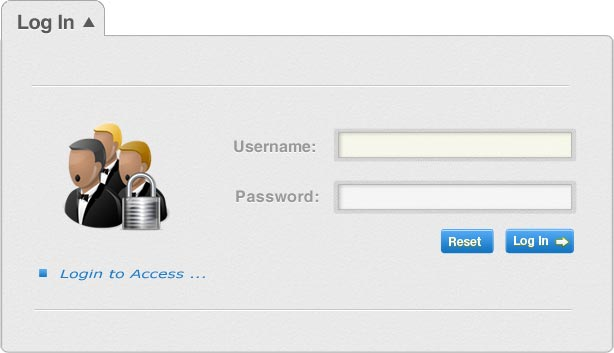
\includegraphics[width=\linewidth]{GUI/Login.jpg}
					\caption{frmDangNhap}
					\label{fig:frmDangNhap}
				\end{figure}
				
%				Vẽ bảng biểu diễn form đăng nhập
					
					\begin{tabular}{|c|c|c| p{5cm}|}
						
						\hline
						STT & Tên Control & Loại Control & Chức năng \\
						\hline
						1 & btLogin & Button & Truyền dữ liệu từ form đăng nhập vào kiểm tra tính hợp lệ trong CSDL. Hiển thị giao diện sử dụng hoặc thông báo đăng nhập thất bại.\\
						\hline
						2 & btReset & Button & Xóa trắc các thông tin trong tại form Đăng nhập, cho phép người dùng nhập lại. \\
						\hline
						
					\end{tabular}
				
%			\newpage
			
			\item Màn hình chính của chương trình
			
				\begin{itemize}
					\item Nhân viên
					
		%			Hình - Màn hình chính của Nhân viên
					\begin{figure}[!h]
						\setlength\fboxsep{1pt}
						\setlength\fboxrule{1pt}
						\fbox{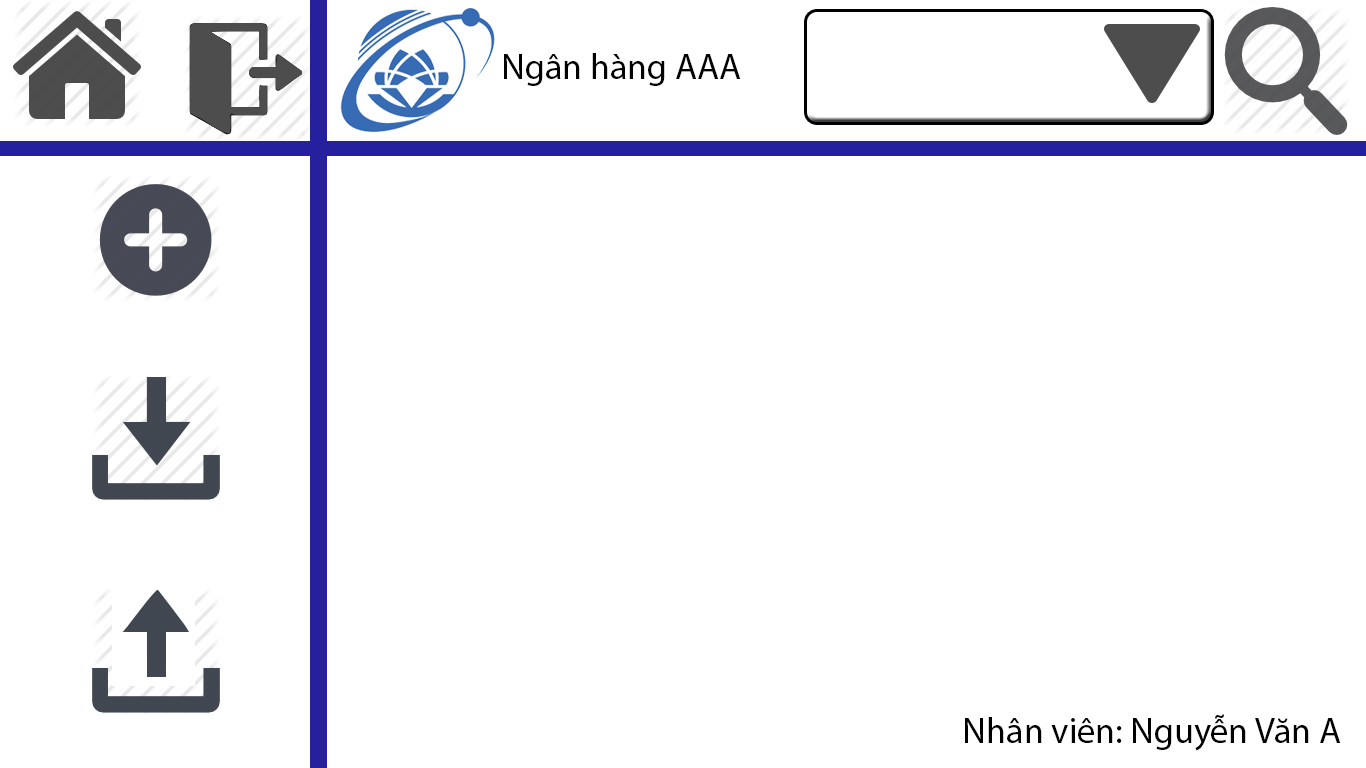
\includegraphics[width=\linewidth]{GUI/MainWND_NV.jpg}}
						\caption{frmManHinhChinhNV}
						\label{fig:frmManHinhChinhNV}
					\end{figure}
					
					% Vẽ bảng biểu diễn form màn hình chính Nhân viên
					
			
	
						\begin{tabular}{|c|c|c|p{5cm}|}
						
						\hline
						STT & Tên Control & Loại Control & Chức năng \\
						\hline
						1 & btHome & Button & Quay trở về màn hình chính\\
						\hline
						2 & btLogout & Button & Đăng xuất khỏi chương trình \\
						\hline
						3 & btAdd & Button & Mở chức năng Lập sổ tiết kiệm \\
						\hline
						4 & btCheckIn & Butoon & Mở chức năng gửi tiền \\
						\hline
						5 & btcheckOut & Button & Mở chức năng rút tiền \\
						\hline
						6 & textboxSearch & TextBox & Nhập thông tin tìm kiếm \\
						\hline
						7 & btSearch & Button & Tìm kiếm theo khóa nhập vào từ TextBox\\
						\hline
						8 & labelUser & Label & Hiển thị thông tin người dùng đang đăng nhập\\
						\hline
					\end{tabular}
			
				
					
					\newpage
					
					\item Quản lý
					
%					Hình - Màn hình chính của Quản lý
					\begin{figure}[!h]
						\setlength\fboxsep{1pt}
						\setlength\fboxrule{1pt}
						\fbox{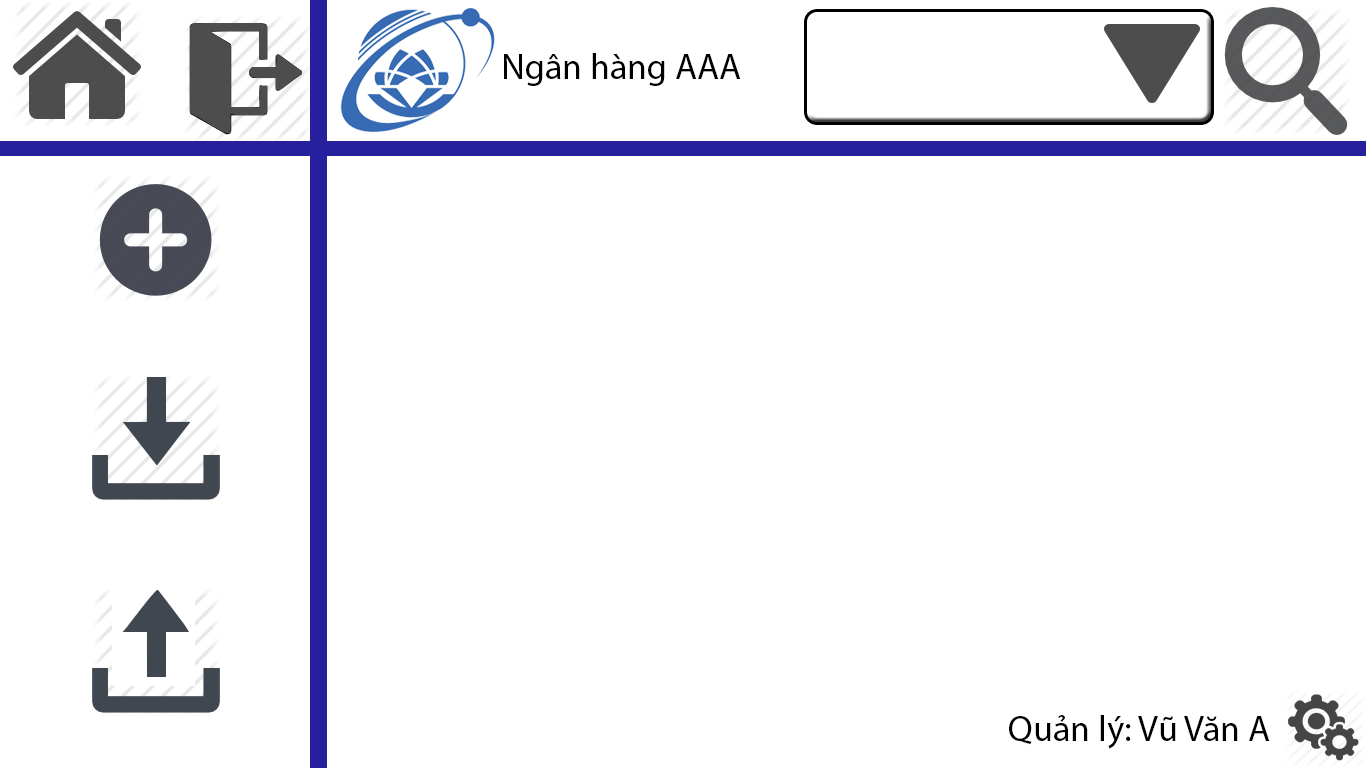
\includegraphics[width=\linewidth]{GUI/MainWND_Boss.jpg}}
						\caption{frmManHinhChinhQL}
						\label{fig:frmManHinhChinhQL}
					\end{figure}
					
					% Vẽ bảng biểu diễn Form Màn hình chính - Quản lý
					\begin{tabular}{|c|c|c| p{5cm}|}
						
						\hline
						STT & Tên Control & Loại Control & Chức năng \\
						\hline
						1 & btHome & Button & Quay trở về màn hình chính\\
						\hline
						2 & btLogout & Button & Đăng xuất khỏi chương trình \\
						\hline
						3 & btAdd & Button & Mở chức năng Lập sổ tiết kiệm \\
						\hline
						4 & btCheckIn & Butoon & Mở chức năng gửi tiền \\
						\hline
						5 & btcheckOut & Button & Mở chức năng rút tiền \\
						\hline
						6 & textboxSearch & TextBox & Nhập thông tin tìm kiếm \\
						\hline
						7 & btSearch & Button & Tìm kiếm theo khóa nhập vào từ TextBox\\
						\hline
						8 & labelUser & Label & Hiển thị thông tin người dùng đang đăng nhập\\
						\hline
						9 & btQuanLy & Button & Chức năng quản lý\\
						\hline
					\end{tabular}
					
				\end{itemize}
			

%			\newpage
			
			\item Các màn hình chức năng
			
				\begin{enumerate}
					\item Màn hình lập sổ
					
%						Hình

						\begin{flushleft}
							\begin{figure}[!h]
								\setlength\fboxsep{1pt}
								\setlength\fboxrule{1pt}
								\fbox{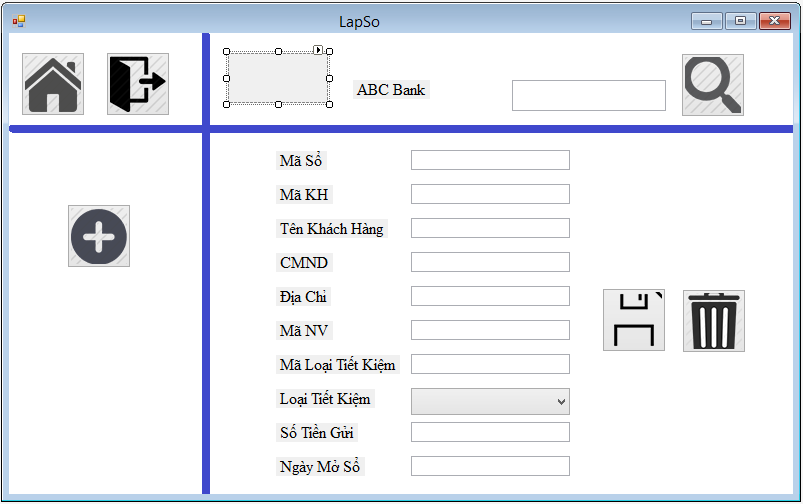
\includegraphics[width=\linewidth]{GUI/Add.png}}
								\caption{frmLapSo}
								\label{fig:frmLapSo}
							\end{figure}
						\end{flushleft}

						\newpage
%						Bảng
						Chi tiết màn hình Lập sổ
						
						\begin{tabular}{|c|c|c| p{5cm}|}
							
							\hline
							STT & Tên Control & Loại Control & Chức năng \\
							\hline
							1 & btHome & Button & Quay trở về màn hình chính\\
							\hline
							2 & btLogout & Button & Đăng xuất khỏi chương trình \\
							\hline
							3 & btAdd & Button & Mở chức năng Lập sổ tiết kiệm \\
							\hline
							6 & textboxSearch & TextBox & Nhập thông tin tìm kiếm \\
							\hline
							7 & btSearch & Button & Tìm kiếm theo khóa nhập vào từ TextBox\\
							\hline
							8 & labelUser & Label & Hiển thị thông tin người dùng đang đăng nhập\\
							\hline
							9 & labelMaSo & Label & Tiêu đề mã sổ \\
							\hline
							10 & textboxMaSo & TextBox & Ô nhập Mã sổ \\
							\hline
							11 & labelMaKhachHang & Label & Tiêu đề Mã khách hàng \\
							\hline
							12 & textboxMaKhachHang & TextBox & Ô nhập Mã khách hàng \\
							\hline
							13 & labelTenKhachHang & Label & Tiêu đề Tên Khách Hàng \\
							\hline
							14 & txtTenKhachHang & TextBox & Ô nhập Tên khách hàng \\
							\hline
							15 & lbCMND & Label & Tiêu đề CMND \\
							\hline
							16 & txtCMND & TextBox & Ô nhập CMND\\
							\hline
							17 & lbDiaChi & Label & Tiêu đề Địa chỉ\\
							\hline
							18 & txtboxDiaChi & TextBox & Ô nhập địa chỉ\\
							\hline
							19 & lbLoaiTietKiem & Label & Tiêu đề Loại Tiết kiệm\\
							\hline
							20 & cboLoaiTietKiem & Checkbox & Hộp chọn Loại tiết kiệm\\
							\hline
							21 & lbSoTienGui & Label & Tiêu đề Số Tiền gửi\\
							\hline
							22 & txtSoTienGui & TextBox & Ô nhập Số tiền gửi\\
							\hline
							23 & lbNgayMoSo & Label & Tiêu đề ngày hết hạn\\
							\hline
							24 & txtNgayMoSo & TextBox & Ô nhập vào ngày mở sổ\\
							\hline
							25 & btSave & Button & Nút lưu sổ\\
							\hline
							26 & btCancel & Button & Nút hủy việc tạo sổ\\
							\hline
						\end{tabular}
						
					\newpage
					
					\item Màn hình gửi tiền
					
					%	Hình
					
						\begin{figure}[!h]
							\setlength\fboxsep{1pt}
							\setlength\fboxrule{1pt}
							\fbox{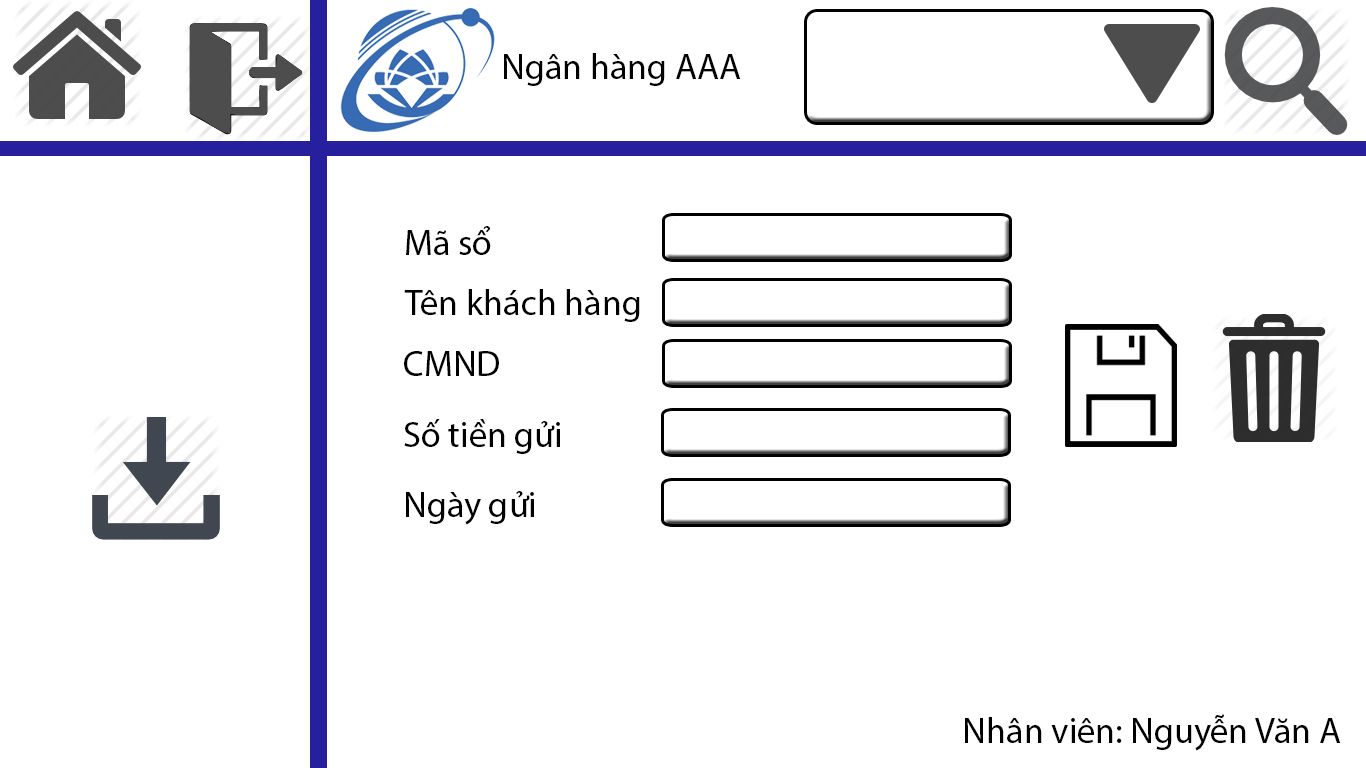
\includegraphics[width=\linewidth]{GUI/GuiTien.jpg}}
							\caption{frmGuiTien}
							\label{fig:frmGuiTien}
						\end{figure}
						
						
						Chi tiết màn hình Gửi tiền
						
						\begin{tabular}{|c|c|c| p{5cm}|}
							
							\hline
							STT & Tên Control & Loại Control & Chức năng \\
							\hline
							1 & btHome & Button & Quay trở về màn hình chính\\
							\hline
							2 & btLogout & Button & Đăng xuất khỏi chương trình \\
							\hline
							3 & btAdd & Button & Mở chức năng Lập sổ tiết kiệm \\
							\hline
							6 & textboxSearch & TextBox & Nhập thông tin tìm kiếm \\
							\hline
							7 & btSearch & Button & Tìm kiếm theo khóa nhập vào từ TextBox\\
							\hline
							8 & labelUser & Label & Hiển thị thông tin người dùng đang đăng nhập\\
							\hline
							9 & btSave & Button & Nút lưu giao dịch gửi tiền\\
							\hline
							10 & btDelete & Button & Nút hủy giao dịch gửi tiền\\
							\hline
							11 & lbMaSo & Label & Tiêu đề mã sổ\\
							\hline
							12 & txtMaSo & Textbox & Ô nhập mã sổ\\
							\hline
							13 & lbTenKH & Label & Tiêu đề tên khách hàng\\
							\hline
							14 & txtTenKH & Textbox & Ô nhập tên khách hàng\\
							\hline
							15 & lbCMND & Label & Tiêu đề hiển thị CMND\\
							\hline
							16 & txtCMND & Textbox & Ô nhập CMND\\
							\hline
							17 & lbSoTienGui & Label & Tiêu đề số tiền gửi\\
							\hline
							18 & txtSoTienGui & Textbox & Ô nhập số tiền gửi\\
							\hline
							19 & lbNgayGui & Label & Tiêu đề ngày gửi\\
							\hline
							20 & txtNgayGui & Textbox & Ô nhập ngày gửi\\
							\hline
						\end{tabular}
					
					\item Màn hình rút tiền
					
					\begin{figure}[!h]
						\setlength\fboxsep{1pt}
						\setlength\fboxrule{1pt}
						\fbox{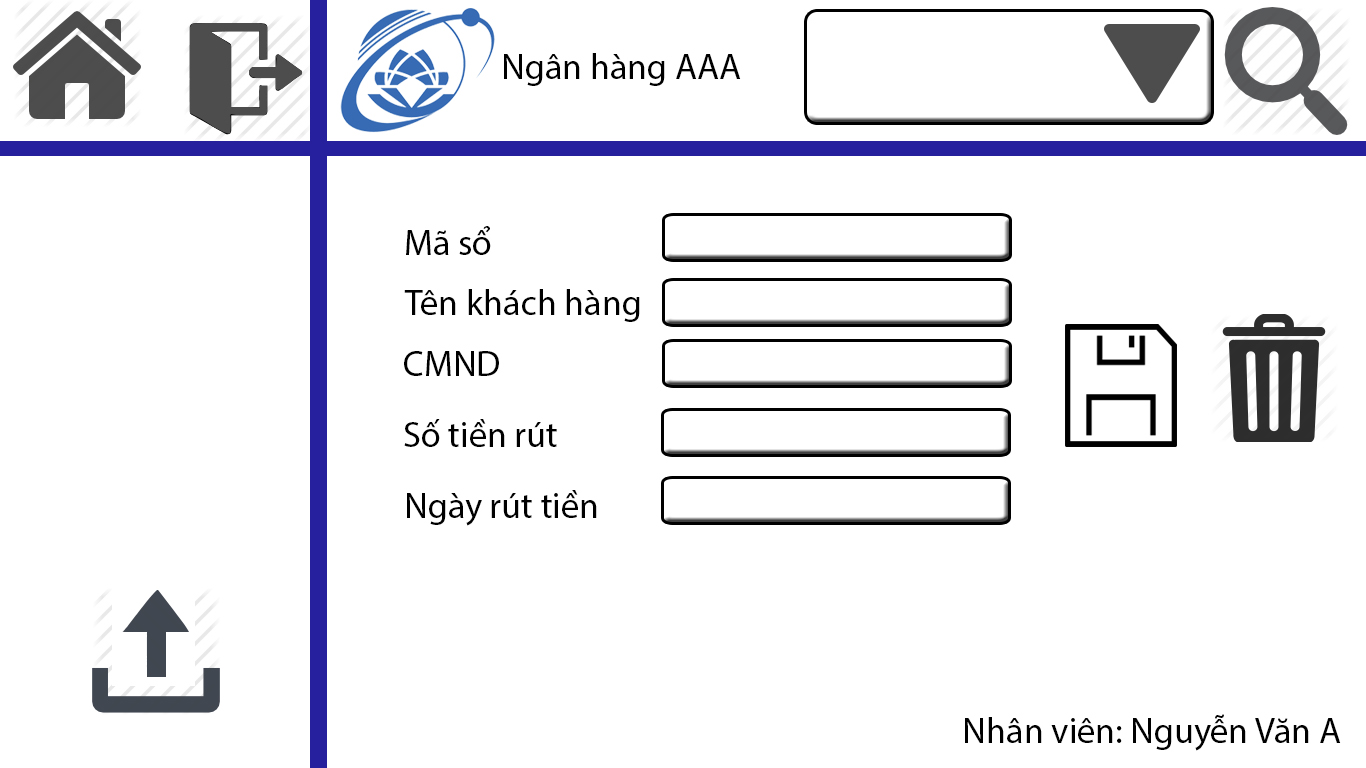
\includegraphics[width=\linewidth]{GUI/RutTien.jpg}}
						\caption{frmRutTien}
						\label{fig:frmRutTien}
					\end{figure}
					
					\begin{tabular}{|c|c|c| p{5cm}|}
						
						\hline
						STT & Tên Control & Loại Control & Chức năng \\
						\hline
						1 & btHome & Button & Quay trở về màn hình chính\\
						\hline
						2 & btLogout & Button & Đăng xuất khỏi chương trình \\
						\hline
						3 & btAdd & Button & Mở chức năng Lập sổ tiết kiệm \\
						\hline
						6 & textboxSearch & TextBox & Nhập thông tin tìm kiếm \\
						\hline
						7 & btSearch & Button & Tìm kiếm theo khóa nhập vào từ TextBox\\
						\hline
						8 & labelUser & Label & Hiển thị thông tin người dùng đang đăng nhập\\
						\hline
						9 & btSave & Button & Nút lưu giao dịch rút tiền\\
						\hline
						10 & btDelete & Button & Nút hủy giao dịch rút tiền\\
						\hline
						11 & lbMaSo & Label & Tiêu đề mã sổ\\
						\hline
						12 & txtMaSo & Textbox & Ô nhập mã sổ\\
						\hline
						13 & lbTenKH & Label & Tiêu đề tên khách hàng\\
						\hline
						14 & txtTenKH & Textbox & Ô nhập tên khách hàng\\
						\hline
						15 & lbCMND & Label & Tiêu đề hiển thị CMND\\
						\hline
						16 & txtCMND & Textbox & Ô nhập CMND\\
						\hline
						17 & lbSoTienRut & Label & Tiêu đề số tiền rút\\
						\hline
						18 & txtSoTienRut & Textbox & Ô nhập số tiền rút\\
						\hline
						19 & lbNgayRut & Label & Tiêu đề ngày rút\\
						\hline
						20 & txtNgayRut & Textbox & Ô nhập ngày rút\\
						\hline
					\end{tabular}
					
				\end{enumerate}
			
			\item Các màn hình thông báo
			
				\begin{itemize}
					\item Thông báo thành công
					
						\begin{figure}[!h]
							\setlength\fboxsep{1pt}
							\setlength\fboxrule{1pt}
							\fbox{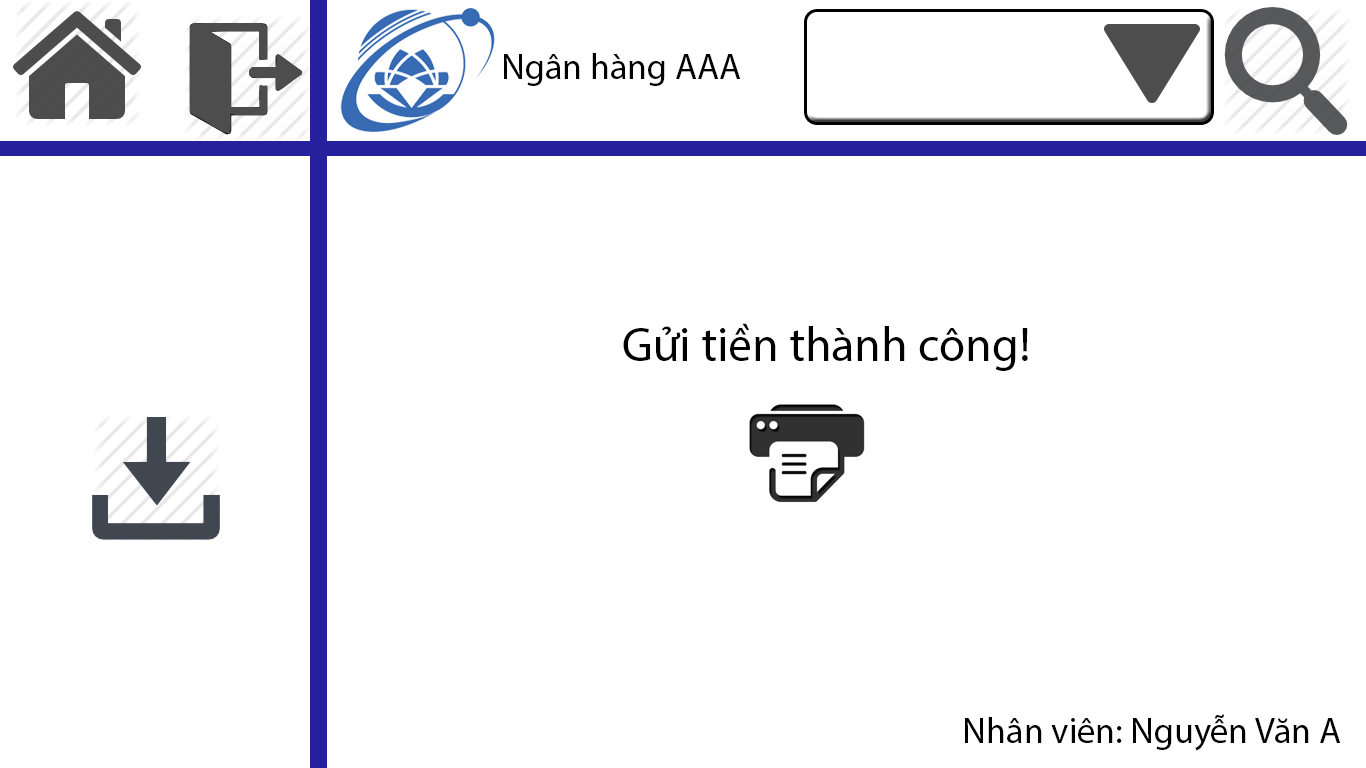
\includegraphics[width=\linewidth]{GUI/GuiTienTC.jpg}}
							\caption{frmGuiTienTC}
							\label{fig:frmGuiTienTC}
						\end{figure}
						
						\begin{tabular}{|c|c|c| p{5cm}|}
							
							\hline
							STT & Tên Control & Loại Control & Chức năng \\
							\hline
							1 & btHome & Button & Quay trở về màn hình chính\\
							\hline
							2 & btLogout & Button & Đăng xuất khỏi chương trình \\
							\hline
							3 & btGuiTien & Button & Mở chức năng gửi tiền \\
							\hline
							6 & textboxSearch & TextBox & Nhập thông tin tìm kiếm \\
							\hline
							7 & btSearch & Button & Tìm kiếm theo khóa nhập vào từ TextBox\\
							\hline
							8 & labelUser & Label & Hiển thị thông tin người dùng đang đăng nhập\\
							\hline
							9 & lbSuccess & Label & Tiêu đê thông báo thành công\\
							\hline
							10 & pbSuccess & PictureBox & Hình ảnh thể hiện việc giao dịch thành công\\
							\hline								
						\end{tabular}
					
					\newpage
					\item Thông báo thất bại
					
					\begin{figure}[!h]
						\setlength\fboxsep{1pt}
						\setlength\fboxrule{1pt}
						\fbox{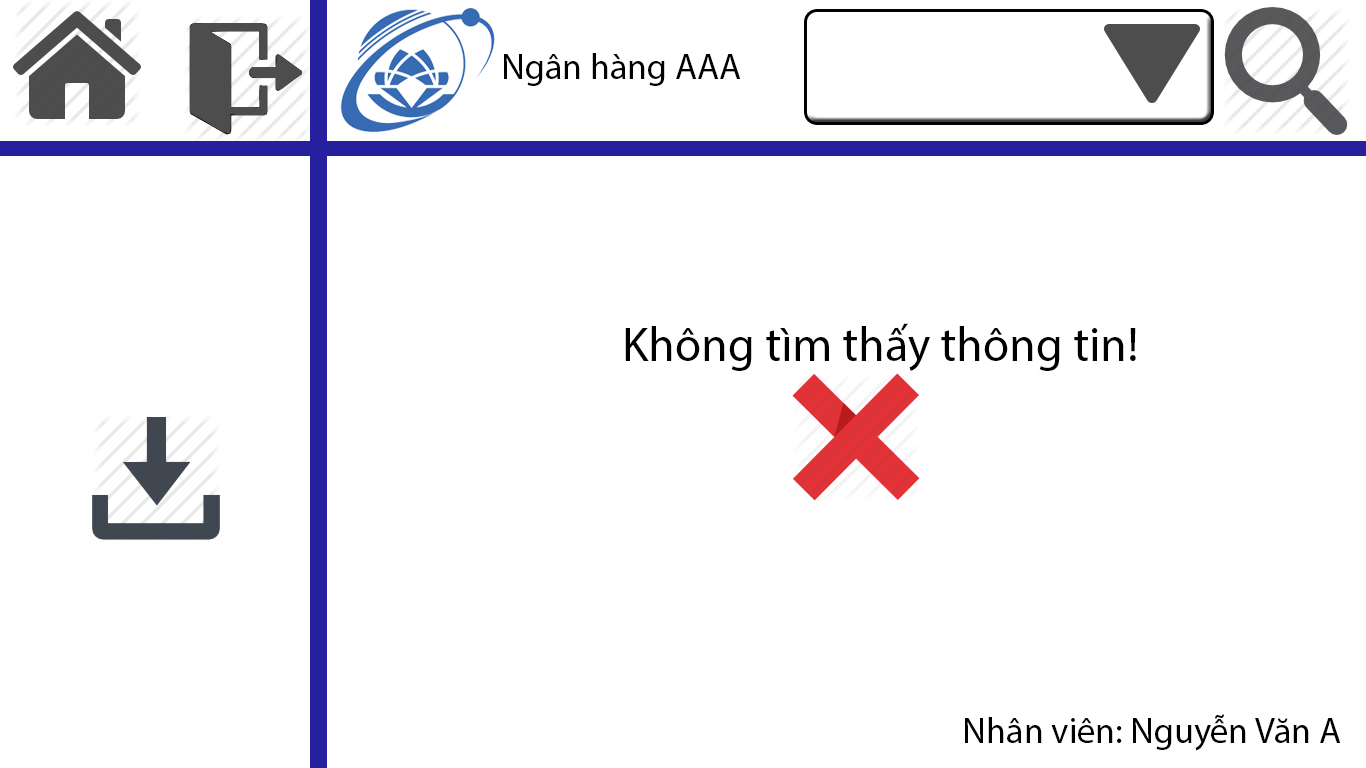
\includegraphics[width=\linewidth]{GUI/GuiTienTB.jpg}}
						\caption{frmGuiTienTB}
						\label{fig:frmGuiTienTB}
					\end{figure}
					
					\begin{tabular}{|c|c|c| p{5cm}|}
						
						\hline
						STT & Tên Control & Loại Control & Chức năng \\
						\hline
						1 & btHome & Button & Quay trở về màn hình chính\\
						\hline
						2 & btLogout & Button & Đăng xuất khỏi chương trình \\
						\hline
						3 & btGuiTien & Button & Mở chức năng gửi tiền \\
						\hline
						6 & textboxSearch & TextBox & Nhập thông tin tìm kiếm \\
						\hline
						7 & btSearch & Button & Tìm kiếm theo khóa nhập vào từ TextBox\\
						\hline
						8 & labelUser & Label & Hiển thị thông tin người dùng đang đăng nhập\\						
						\hline
						9 & lbFail & Label & Tiêu đê thông báo thất bại\\
						\hline
						10 & pbFail & PictureBox & Hình ảnh thể hiện việc giao dịch thất bại\\
						\hline						
					\end{tabular}
					
					\newpage
					\item Màn hình thống kê - quản lý
						\begin{figure}[!h]
							\setlength\fboxsep{1pt}
							\setlength\fboxrule{1pt}
							\fbox{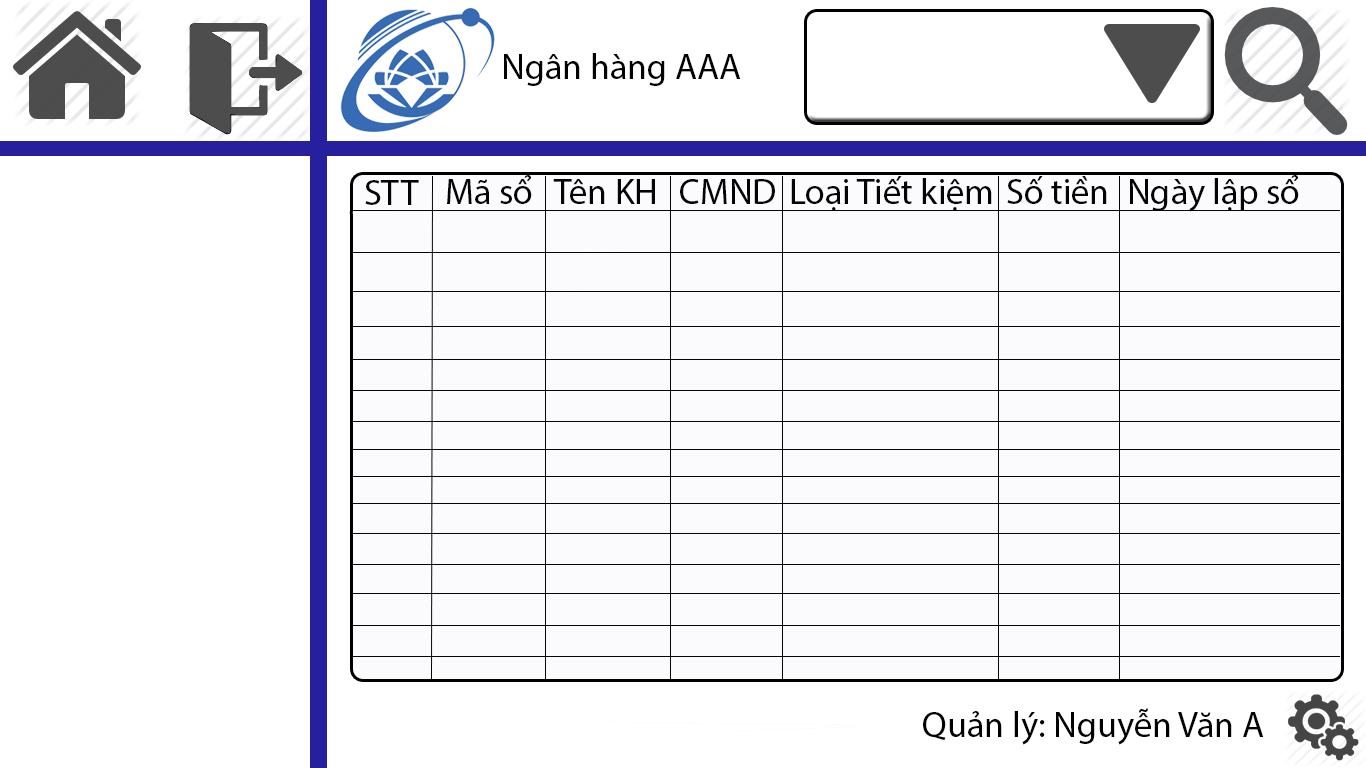
\includegraphics[width=\linewidth]{GUI/Manage.jpg}}
							\caption{frmThongKe}
							\label{fig:frmThongKe}
						\end{figure}
				\end{itemize}
			
		\end{enumerate}
	
	
	\section{Thiết kế dữ liệu}
		\subsection{Thiết kế dữ liệu}
			\begin{itemize}
				\item KHACHHANG (\underline{MaKH}, HoTen, CMND, DiaChi, NgSinh, NgDangKy)
				\item NHANVIEN (\underline{MaNV}, HoTen, CMND, DiaChi, NgSinh, ChucVu, Luong)
				\item CACLOAITIETKIEM (\underline{MaLTK}, LoaiTietKiem, LaiSuat, SoTienGuiMin, SoNgayGuiMin)
				\item SOTIETKIEM (\underline{MaSTK}, MaKH, MaNV, MaLTK, SoTienGui, NgMoSo)
				\item PHIEUGUITIEN (\underline{MaPhieu}, MaSTK, MaNhanVienGD, NgGui, SoTien)
				\item PHIEURUTTIEN (\underline{MaPhieu}, MaSTK, MaNhanVienGD, NgRut, SoTien)
			\end{itemize}
			
%			\newpage
			\begin{center}				
				\begin{tabular}{|l|l|l|l|p{4.5cm}|}
					\hline
					STT & Thuộc tính & Kiểu dữ liệu & Giá trị khởi động & Ràng buộc\\
					\hline
					1 & CMND & char(9) & NULL & \parbox[t]{4.5cm}{Not NULL\\ Không được là chữ\\ Không được dài quá 9 chữ số} \\
					\hline
					2 & LoaiTietKiem & varchar(30) & NULL & \parbox[t]{4.5cm}{Chỉ được là 1 trong 3 chính sách hợp lệ}\\
					\hline
					3 & SoTienGui & money & & \parbox[t]{4.5cm}{Lớn hơn 100000}\\
					\hline					
				\end{tabular}
			\end{center}
			
	\subsection{Mô hình vật lý}
		\begin{figure}[!h]
			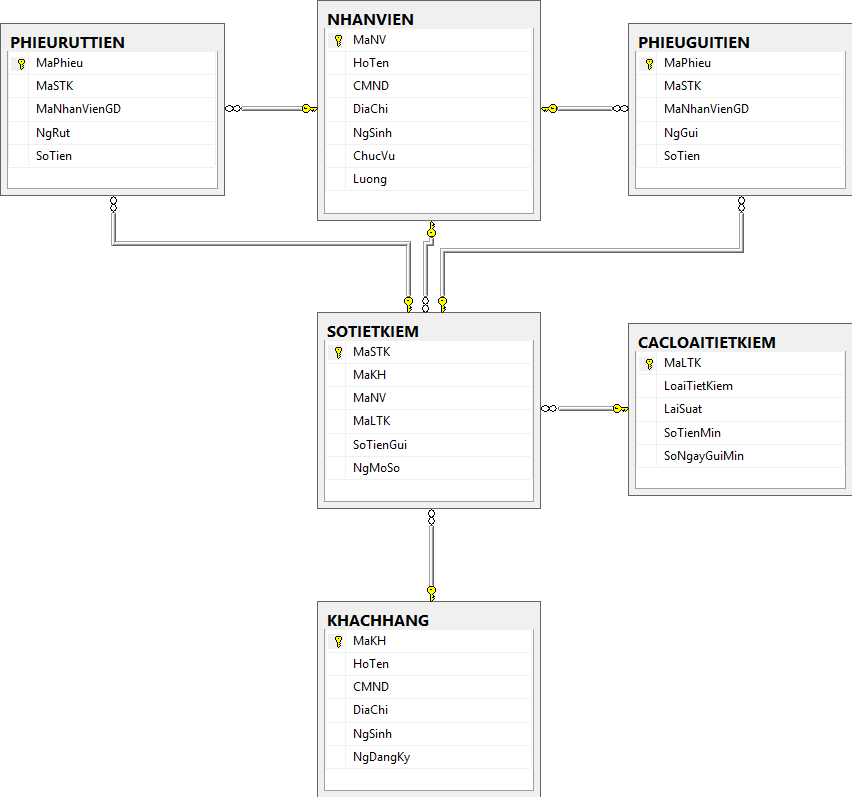
\includegraphics[width=\linewidth]{GUI/SQL.png}
			\caption{Relational Data Modeling}
			\label{fig:RDM}
		\end{figure}
	\section{Mô hình và thiết kế xử lý}
		\subsection{Danh sách các hàm xử lý}
		
			\begin{tabular}{|c|c|c|p{4.5cm}|}
				\hline
				STT & Mã xử lý & Tên xử lý & Mô tả\\
				\hline
				1 & XL1 & Mở sổ tiết kiệm & Mở sổ tiết kiệm khi khách hàng mới gửi tiền lần đầu\\
				\hline
				2 & XL2 & Lưu và in sổ tiết kiệm & Lưu thông tin của khách hàng xuống CSDL, thông báo kết quả của việc lưu và in sổ ra cho khách hàng\\
				\hline
				3 & XL3 & Lập phiếu gửi tiền & Lập phiếu gửi khi khách hàng muốn gửi tiền vào sổ tiết kiệm\\
				\hline
				4 & XL4 & Lưu phiếu gửi tiền & Lưu thông tin của khách hàng xuống CSDL và in ra cho khách hàng\\
				\hline
				5 & XL5 & Lập phiếu rút tiền và lưu in & Khi khách hàng muốn rút tiền trong sổ ra lập phiếu rút tiền, lưu thông tin xuống CSDL và in ra cho khách hàng\\
				\hline
				6 & XL6 & Tra cứu sổ & Cho phép tìm kiếm thông tin của một sổ để xem, cập nhật thông tin\\
				\hline
				7 & XL7 & Lập báo cáo ngày & Báo cáo thu chi số lượng tiền rút ra và thu vào trong ngày\\
				\hline
				8 & XL8 & Lập báo cáo tháng & Báo cáo thu chi số lượng tiền trong tháng.\\
				\hline
			\end{tabular}
		
		\subsection{Mô tả chi tiết các xử lý}
		
			\begin{itemize}
				\item Màn hình lập sổ
				
					\begin{tabular}{|c|c|c|p{1.5cm}|}
						\hline
						STT & Biến cố & Xử lý & Mã xử lý\\
						\hline
						1 & Nút Lưu & Lưu toàn bộ thông tin nhân viên mới nhập xuống CSDL & XL1\\
						\hline
						2 & Nút Hủy & Xóa trắng form và hủy thao tác thêm sổ & XL2\\
						\hline
						3 & Nút Tìm kiếm & Tìm thông tin về sổ trong CSDL & XL3\\
						\hline
						4 & Nút Đăng xuất & Thoát khỏi chương trình & XL4\\
						\hline
					\end{tabular}
				
				\item Màn hình chính
				\item Màn hình rút tiền
				\item Màn hình gửi tiền
				
			\end{itemize}
	
		\section{Kế hoạch lập trình và kiểm thử đơn vị}
			\subsection{Môi trường lập trình}
				\begin{itemize}
					\item IDE: Visual Studio 2013 Ultimate
					\item Ngôn ngữ lập trình: C\#
					\item Thư viện phụ thuộc: .Net framework 4.5
					\item Sử dụng SVN để quản lý phiên bản. (Google Code + Tortoise svn client)
				\end{itemize}
				
			\subsection{Phương pháp lập trình}
			
				\begin{itemize}
					\item Hướng đối tượng, các đối tượng chính:
					
						\begin{itemize}
							\item Nhân viên
							\item Sổ tiết kiệm
							\item Khách hàng
							\item Chính sách tiết kiệm
						\end{itemize}
					\item Phương pháp tiếp cận Top - Down
					
						\begin{itemize}
							\item Khái quát chương trình cần quản lý sổ tiết kiệm của khách hàng, cho phép thực hiện các thao tác \textit{Tạo sổ, Gửi tiền, Rút tiền.}
							\item 2 mức nhân viên: \textit{NV thường, NV quản lý}
							\item Các chính sách tiết kiệm
							
								\begin{itemize}
									\item Không kỳ hạn
									\item Kỳ hạn 3 tháng
									\item Kỳ hạn 6 tháng
								\end{itemize}
							
						\end{itemize}
					
				\end{itemize}
			
			\subsection{Tổ chức kiến trúc chương trình}
			
				\begin{itemize}
					\item Sử dụng mô hình 3 lớp
					
						\begin{itemize}
							\item GUI: Sử dụng form C\# để thiết kế giao diện
							\item Logic: xử lý các yêu cầu, ràng buộc của chương trình
							\item CSDL: lưu trữ thông tin của các bảng gồm thông tin người dùng, thông tin sổ tiết kiệm, lịch sử giao dịch.
						\end{itemize}
					
					\item Triển khai trên máy local - 1 tầng
				\end{itemize}
			
			\subsection{Quản lý version}
			
				\begin{itemize}
					\item SVN để quản lý phiên bản code
					\item http://da-cnpm-uit-se7.googlecode.com/svn/trunk/
					\item Git để quản lý phiên bản báo các và tài liệu
					\item https://github.com/vunhan/CNPM
				\end{itemize}
			
			\subsection{Chuẩn viết mã}
			
				\begin{itemize}
					\item Cách đặt tên
					
						\begin{itemize}
							\item Tên các form được thiết kế \textit{frmTenForm}
							\item Tương tự với tên biến, button (bt), label (lb), Textbox (txt), PictureBox (pb)
						\end{itemize}
%					\newpage
					\item Bố cục
					
						\begin{itemize}
							\item Sử dụng các cấu hình mặc định của VS editor (canh lề thông minh, dùng tab thay vì space)
							\item Viết một biểu thức trên 1 dòng
							\item Viết mỗi miêu tả trên một dòng
							\item Thêm tối thiểu 1 dòng trắng giữa các khai báo và định nghĩa phương thức 
							\item Dùng các dấu ngoặc đơn để phân chia các biểu thức toán học một cách rõ ràng.
						\end{itemize}
					
					\item Chú thích
					
						\begin{itemize}
							\item Viết comment ra một dòng riêng, không được đặt vào cuối dòng code.
							\item Bắt đầu dòng comment với kí từ đầu viết hoa
							\item Không sử dụng block comment, sử dụng các // riêng lẻ
						\end{itemize}
				\end{itemize}
			
			\subsection{Kiểm thử}
			
				\begin{enumerate}
					\item Các yêu cầu của quá trình kiểm thử
					
						\begin{itemize}
							\item Phần mềm đã đáp ứng được yêu cầu của bản đặc tả yêu cầu hay chưa?
							\item Thực hiện công việc như mong đợi hay không?
							\item Cơ chế sao lưu dữ liệu
							\item Bảo mật CSDL
							\item Các dữ liệu được ràng buộc một cách chặt chẽ
						\end{itemize}
					
				\end{enumerate}
		
	\section{Phân công công việc}
	
		\begin{itemize}
			\item Khảo sát hiện trạng và đặc tả yêu cầu: Hiếu
			\item Thiết kế giao diện: Nhân
			\item Thiết kế dữ liệu: Hùng
			\item Thiết kế xử lý: Hiếu
			\item Soạn chuẩn viết mã: Nhân
			\item Lập trình: Hiếu + Hùng
			\item Tổng hợp báo cáo: Nhân
			
		\end{itemize}
			
%	\newpage			
	\section{Kết luận}
		
		\subsection{Bài học}
		
			\begin{itemize}
				\item Làm quen một số quy trình phát triển phần mềm phổ biến
				\item Nắm vững quy trình phát triển phần mềm Thác nước - ứng dụng vào đồ án môn học
				\item Ôn tập lại kiến thức về thiết kế CSDL, lập trình C\#
				\item Làm quen với các kỹ thuật khảo sát, phân tích, viết đặc tả yêu cầu
				\item Biết cách thiết kế giao diện một cách trực quan, nắm được một số yêu cầu cơ bản trong thiết kế giao diện
				\item Biết cách sử dụng và có cơ hội luyện tập sử dụng các hệ thống quản lý phiên bản (GIT vs SVN)
				\item Kỹ năng làm việc nhóm
				\item Sử dụng LaTex để viết báo cáo tổng hợp.
			\end{itemize}
		
		\subsection{Khuyết điểm}
			\begin{itemize}
				\item Tài liệu thiết kế xử lý chưa hoàn chỉnh.
				\item Tài liệu thiết kế dữ liệu bị xung đột với phần thiết kế giao diện.
				\item Kế hoạch lập trình không tiến hành đúng tiến độ -> Không thể qua bước kiểm thử
				\item Phân công công việc chưa hợp lý, quản lý tiến độ không sát sao dẫn đến việc công đoạn lập trình chưa hoàn thành.
				\item Đa số thành viên còn gặp khó khăn trong việc sử dụng SVN và merge code dẫn đến việc thất lạc code và sử dụng SVN không thật sự hiệu quả.
			\end{itemize}
		\subsection{Kinh nghiệm}
		
			\begin{itemize}
				\item Tiến hành cài đặt và hướng dẫn sử dụng các công cụ hỗ trợ lập trình sớm.
				\item Phân công công việc hợp lý và tiến hành giám sát tiến độ sát sao hơn.
				\item Sớm phát hiện các khó khăn trong nhóm và hỗ trợ nhau.
			\end{itemize}
		
\end{document}}